\subsection{The Individual Decision Problem}

\begin{figure}
	\centering
	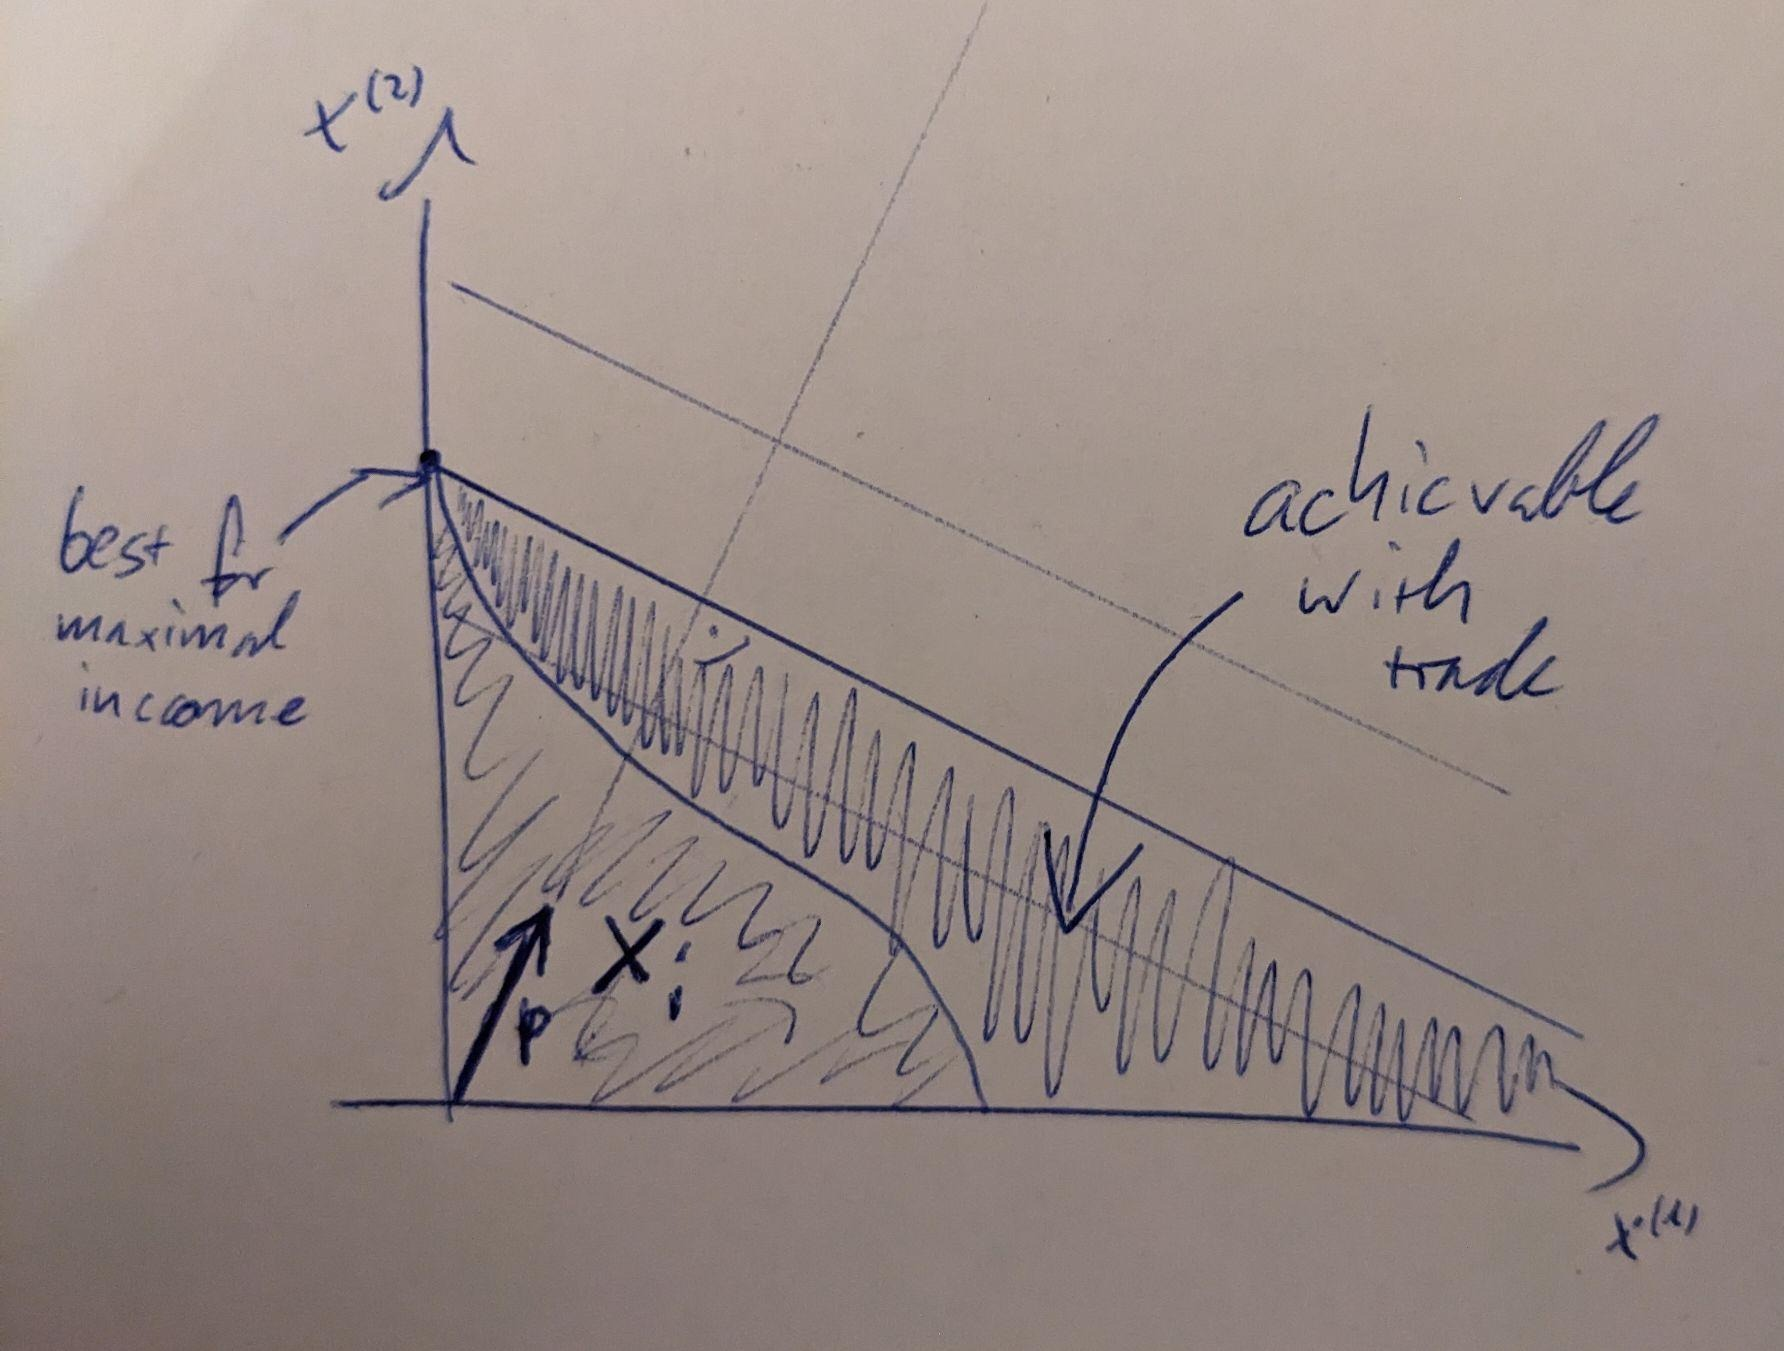
\includegraphics[width=0.7\textwidth]{images/consumption_increase_by_trade.jpeg}
	\caption{
		Product vectors on the \(d-1\) dimensional hyperplanes orthogonal to \(p\)
		cost the same amount and can therefore be exchanged (here \(d=2\), so the
		hyperplanes are lines). Trading at prices \(p\) enlarges the set of
		product vectors available for consumption for person \(i\).
	}
	\label{fig: consumption increase by trade}
\end{figure}
For a fixed price vector \(p\), let us consider the production and consumption
decision of person \(i\). As their expenses have to be smaller than their
income, it makes sense to maximize income for a given amount of labour \(L_i\).
Recall that our production options are \(X_i=X_i(L_i)\). So the maximal income
given labour \(L_i\) is
\[
	\tag{income}\label{eq: income}
	\mu(p, X_i) := \sup\{\langle p, x\rangle : x\in X_i\}.
\]
The function \(\mu(\cdot, X_i)\) in \(p\), is called the ``support function'' of
\(X_i\). It has some useful properties we will be grateful for later on. The
individual decision problem of person \(i\) therefore becomes
\begin{equation}
	\tag{IDP}
	\label{eq: individual decision problem}
	\max_{L_i, y} u(1-L_i, y) \quad\text{s.t.}\quad
	\langle y, p\rangle \le \mu(p, X_i(L_i))
\end{equation}
In Figure~\ref{fig: consumption increase by trade} we can see, how this
constraint is always weaker than \(y\in X_i(L_i)\), which is the constraint of
self-sufficiency. I.e. we get the following lemma.

\begin{lemma}[Trade is never harmful]
\[
	\underbrace{X_i(L_i)}_{\text{own production}}
	\subseteq \quad \conv(X_i)\quad
	\subseteq \quad
	\underbrace{
		\{y\in\real_{\ge 0}^\dims: \langle y, p\rangle \le \mu(p, X_i)\}
	}_{\text{consumption options with trade}}
\]
\end{lemma}
\begin{proof}
	Choose an arbitrary \(y\in \conv(X_i)\). Then there exist \(y_1,\dots, y_m\in X_i\)
	such that \(y=\sum_{k=1}^m \lambda_k y_k\) for \(\lambda_k\in[0,1]\) with
	\(\sum_{k=1}^{m}\lambda_k=1\). Then by definition of \(\mu\)
	\[
		\langle p, y\rangle
		= \sum_{k=1}^m \lambda_k\langle p, y_k\rangle
		\overset{y_k\in X_i}\le \underbrace{\sum_{k=1}^m \lambda_k}_{=1}
		\sup\{\langle p, x\rangle : x\in X_i\}
		\overset{\text{def.}}= \mu(p, X_i).
	\]
	So \(y\) is a consumption option with trade.
\end{proof}

\subsubsection{Income in the Pure Variable Cost Case}

\begin{lemma}[Income in the Pure Variable Cost Case]
	\label{lem: income in the pure variable cost case}
	In the pure variable cost case \(L_i(x) = \langle l_i, x\rangle\), income
	can be written as
	\[
		\mu(p, X_i(L_i))
		= \overbrace{L_i}^{\text{work time}} \max_{j=1,\dots,\dims}
		\underbrace{\frac{p_j}{l_i^{(j)}}}_{=: w_i^{(j)}}
		= L_i \overbrace{\|w_i\|_\infty}^{\text{wage}},
	\]
	where \(w_i^{(j)}\) are potential wages for producing good \(j\).
\end{lemma}
\begin{proof}
	Let \(H:= \diag(l_i)\), then as \(X_i\) is compact we know the supremum is
	a maximum and
	\begin{align*}
		\mu(p, X_i)
		&= \max_{x\ge 0} \langle p, x\rangle
		\text{ s.t. } \langle x, l_i\rangle \le L_i\\
		&\overset{y=Hx}= \max_{y\ge 0} \langle p, H^{-1}y\rangle
		\text{ s.t. } \underbrace{\langle H^{-1}y, l_i\rangle}_{
			= \langle y, 1 \rangle = \|y\|_1
		} \le L_i\\
		&= L_i \underbrace{
			\max_{y\ge 0} \langle H^{-1}p, y\rangle \text{ s.t. } \|y\|_1 \le 1
		}_{
			= \|H^{-1} p\|_{\text{Op-Norm(1)}} = \|H^{-1} p \|_\infty
		}\\
		&= L_i \max_{j=1,\dots,\dims} \frac{p_j}{l_i^{(j)}},
	\end{align*}
	where we have used, that all entries of \(y\) are non-negative when
	converting to the \(1\)-norm, \(\|x\|_1 = \sum_{i=1}^\dims |x_i|\), the
	fact that the operator norm of the \(1\)-norm is the sup norm
	\(\|x\|_\infty = \sup_{i=1,\dots,\dims} |x_i|\)\fxnote{source or appendix},
	and finally positivity of entries of \(p\) and \(l_i\) again.
\end{proof}

\subsubsection{Income with Fixed Costs}

While the pure variable cost case already lends itself to specialization, unless
multiple wage options \(w_i^{(j)}\) are identical, adding fixed costs truly
encourages specialization. For fixed costs \(f_i\) the production capability
of person \(i\) can be written as 
\[
	X_i = \{
		x\in \real_{\ge 0}^\dims
		: \langle l_i, x\rangle
		+ \underbrace{
			\sum_{j=1}^\dims f_i^{(j)}\ind_{x^{(j)}>0}
		}_{=: \langle f_i, \ind_{>0}\rangle} \le L_i
	\}.
\]

\begin{lemma}[Income in Variable \& Fixed Cost Case]
	\label{lem: income in mixed case}
	We assume the person is able to produce any product. So none of the fixed
	costs \(f_i^{(j)}\) take longer than the total labour time \(L_i\) (i.e.
	\(L_i - f_i^{(j)} > 0\)). In this mixed case, income of person \(i\) can be
	written as		
	\[
		\mu(p, X_i)
		= L_i \max_{j=1,\dots,d}
		\underbrace{\frac{p_j}{\bar{l}_i^{(j)}}}_{=:w_i^{(j)}}
		= L_i \|w_i\|_\infty,
	\]
	where the average labour cost \(\bar{l}_i^{(j)}\) of person \(i\) of
	specialization \(j\) is given by
	\[
		\bar{l}_i^{(j)}
		:= l_i^{(j)}\frac{L_i}{L_i-f_i^{(j)}}
		= l_i^{(j)}\frac{1}{1-f_i^{(j)}/L_i}
	\]
\end{lemma}
\begin{proof}
	For a subset \(J\subseteq\{1,\dots,\dims\}\) define the subspace
	\[
		\real_{>0}^J:= \{
			x\in \real^\dims:
			x^{(j)} > 0\ \forall j\in J;\;\; x_j =0\ \forall j\notin J
		\}.
	\]
	Then we can partition our maximization problem by these \(J\) like this:
	\begin{align*}
		\mu(p, X_i)
		&= \max_{x\ge 0}\langle p, x\rangle \text{ s.t. }
		\langle x, l_i\rangle  + \langle f_i, \ind_{>0}\rangle \le L_i\\
		&= \max_{J \subseteq \{1,\dots,\dims\}}
		\max_{x\in \real_{>0}^J}
		\langle p, x\rangle \text{ s.t. }
		\langle x, l_i\rangle \le L_i - \sum_{j\in J}f_i^{(j)}
	\end{align*}	
	We can relax the inner maximization problem to obtain the pure variable
	optimization problem embedded in \(\real^I\)
	\begin{align*}
		&\max_{x\in \real_{>0}^J}
		\langle p, x\rangle \text{ s.t. }
		\langle x, l_i\rangle \le L_i - \sum_{j\in J}f_i^{(j)}\\
		&\le 
		\max_{x\in \real_{{\color{red} \ge} 0}^J}
		\langle p, x\rangle \text{ s.t. }
		\langle x, l_i\rangle \le L_i - \sum_{j\in J}f_i^{(j)}\\
		&= \Bigl(L_i - \sum_{j\in J}f_i^{(j)}\Bigr)
		\max_{j\in J} \frac{p_j}{l_i^{(j)}}
	\end{align*}
	So in total, we have
	\begin{align*}
		\mu(p, X_i)
		&\le \max_{\emptyset \neq J\subseteq \{1,\dots,\dims\}}
		\Bigl(L_i - \sum_{j\in J}f_i^{(j)}\Bigr)
		\max_{j\in J} \frac{p_j}{l_i^{(j)}}\\
		&= \max_{j=1,\dots,\dims}
		(L_i - f_i^{(j)}) \frac{p_j}{l_i^{(j)}}.
	\end{align*}
	To see that this upper bound is actually tight, consider producing
	exclusively \(j\). Then we have
	\[
		l_i^{(j)} x^{(j)} + f_i^{(j)} = L_i \iff x^{(j)}
		= \frac{L_i-f_i^{(j)}}{l_i^{(j)}}.
	\]
	Optimizing over different specializations yields
	\[
		\mu(p, X_i) \ge \max_{j=1,\dots,\dims} p_j x^{(j)}
		= \max_{j=1,\dots,\dims}
		p_j \frac{L_i - f_i^{(j)}}{l_i^{(j)}}
		= L_i\max_{j=1,\dots,\dims}
		\frac{p_j}{l_i^{(j)}\frac{L_i}{L_i - f_i^{(j)}}}.
	\]
	Lastly the average labour cost of specialization \(j\) is given by
	\begin{align*}
		\bar{l}_i^{(j)}
		&= \frac{L_i}{x^{(j)}}
		= \frac{l_i^{(j)} x^{(j)} + f_i^{(j)}}{x^{(j)}}
		= l_i^{(j)} + \frac{f_i^{j}}{\left(\frac{L_i-f_i^{(j)}}{l_i^{(j)}}\right)}
		= l_i^{(j)} \Bigl[1 + \frac{f_i^{j}}{L_i-f_i^{(j)}}\Bigr]\\
		&=l_i^{(j)}\frac{L_i}{L_i - f_i^{(j)}}.
		\qedhere
	\end{align*}
\end{proof}

\subsubsection{The Individual Decision Problem in the Mixed Case}

By talking about average costs \(\bar{l}_i^{(j)}\) in place of variable costs
\(l_i^{(j)}\), we salvaged the results from the pure variable
cost case. But no matter how the wage \(\|w_i\|_\infty\) comes to be, the
individual decision problem \eqref{eq: individual decision problem} becomes
\[
	\max_{L_i, y} u(1-L_i, y) \text{ s.t. } \langle p, y\rangle \le L_i \|w_i\|_\infty
\]
or in other words
\[
	\max_{y} u\left(1- \frac{\langle p, y\rangle}{\|w_i\|_\infty}, y\right).
\]
The first order condition is therefore
\[
	\frac{du}{dy} 
	= u_f\Bigl[
		\underbrace{\frac{u_y}{u_f}}_{\text{wtw}}
		- \overbrace{\frac{p}{\|w_i\|_\infty}}^{\text{effort required}}
	\Bigr]
	= \frac{u_f}{\|w_i\|_\infty}\Bigl[
		\underbrace{\frac{u_y}{u_f}\|w_i\|_\infty}_{\wtp}
		- p
	\Bigr]
\]
Where the ``willingness to pay'' (wtp) is simply the willingness to work
(wtw) scaled by person \(i\)'s wages.

Careful readers might have noticed, that
this calculation is not quite accurate in the mixed case. Because the average
costs depend on \(L_i\), which in turn makes \(\|w_i\|_\infty\) dependent on
\(L_i\). So by the product rule, the effort required would be
\[
		\frac{dL_i}{dy}
		= \frac{d}{dy} \frac{\langle p, y\rangle}{\|w_i\|_\infty}
		= \frac{p}{\|w_i\|_\infty}
		- \frac{\langle p, y\rangle}{\|w_i\|_\infty^2}
		\frac{d\|w_i\|_\infty}{dL_i}\frac{dL_i}{dy}
\]
Joining the \(\frac{dL_i}{dy}\) on both sides results in
\[
	\frac{dL_i}{dy}
	= \frac{\frac{p}{\|w_i\|_\infty}}{
		1 + \frac{\langle p, y\rangle}{\|w_i\|_\infty^2}
		\frac{d\|w_i\|_\infty}{dL_i}
	}
	= \frac{p}{
		\|w_i\|_\infty + \frac{\langle p, y\rangle}{\|w_i\|_\infty}
		\frac{d\|w_i\|_\infty}{dL_i}
	}.
\]
Where \(\|w_i\|_\infty=\max_{j} w_i^{(j)}\) is piecewise differentiable with
derivatives
\[
	\frac{dw_i^{(j)}}{dL_i}
	= \frac{d}{dL_i} \frac{p_j}{\bar{l}_i^{(j)}}
	= \frac{p_j}{l_i^{(j)}} \frac{d}{dL_i} \frac{L_i-f_i^{(j)}}{L_i}
	= \frac{p_j}{l_i^{(j)}} \frac{f_i^{(j)}}{L_i^2} > 0.
\]
In other words: Wages increase with total labour time \(L_i\), as
average cost decrease with \(L_i\). The size of this effect increases with the
size of the fixed costs. If the fixed costs are close to \(L_i\) small decreases
of \(L_i\) might make producing \(j\) completely unviable, but at the very least
cut heavily into the little time left for actually producing \(j\). In fact
average costs have singularities at \(f_i^{(j)}\)
\[
	\lim_{L_i\downarrow f_i^{(j)}} \bar{l}_i^{(j)}
	= \lim_{L_i\downarrow f_i^{(j)}}l_i^{(j)}\frac{1}{1-f_i^{(j)}/L_i}
	= \infty.
\]
Using \(\bar{l}_i^{(j)}=l_i^{(j)}\frac{L_i}{L_i-f_i^{(j)}}\) we can alternatively
write
\[
	\frac{dw_i^{(j)}}{dL_i}
	= \frac{p_j}{\bar{l}_i^{(j)}} \frac{f_i^{(j)}(L_i-f_i^{(j)})}{L_i}
	= w_i^{(j)} \frac{f_i^{(j)}(L_i-f_i^{(j)})}{L_i}.
\]
With \(j^* := \argmax_{j} w_i^{(j)}\) and \(L_i = \frac{\langle p,
y\rangle}{\|w_i\|_\infty}\), this finally results in the effort required
\[
	\frac{dL_i}{dy}
	= \frac{p}{
		\|w_i\|_\infty + \langle p, y\rangle f_i^{(j^*)}
		\bigl(1-\frac{f_i^{(j^*)}}{L_i}\bigr)
	}
	= \frac{p}{
		\|w_i\|_\infty + f_i^{(j^*)}
		\bigl(\langle p, y\rangle-f_i^{(j^*)}\|w_i\|_\infty\bigr)
	}.
\]
The willingness to pay is therefore given by
\[
	\wtp = \frac{u_y}{u_f}\Bigl[
		\|w_i\|_\infty + f_i^{(j^*)}
		\bigl(\langle p, y\rangle-f_i^{(j^*)}\|w_i\|_\infty\bigr)
	\Bigr].
\]
